\documentclass[11pt, compress, aspectratio=1610]{beamer}

\usetheme{pl}

% Set language
\usepackage{xstring}
\newcommand{\Langue}[1]{%
    \IfEqCase{#1}{%
        {francais}{
        \usepackage[utf8]{inputenc}
        \usepackage[francais]{babel}
        }%
        {english}{\usepackage[english]{babel}}%
    }[\PackageError{Langue}{Undefined option to language: #1}{}]%
}%
\Langue{francais}

% tikz diagrams
\usepackage{tikz}
\usetikzlibrary{shapes,snakes}
\usetikzlibrary{er}
\usetikzlibrary{arrows, plotmarks, decorations.markings}
\tikzstyle{arrow} = [->,>=stealth,thick,rounded corners=10pt,line width=0.1pt]
\usetikzlibrary{shadows}
\usetikzlibrary{shadings}
\usetikzlibrary{tikzmark, positioning, calc} % calc, to calculate coordinate
\tikzstyle{State}=[circle,
		thick,
		minimum size = 0.8cm,
		inner sep =5pt,
		draw=plST,
		fill=plST]

\usepackage{verbatim}
\usepackage{longtable}
\usepackage{booktabs}
\usepackage{minted}
\usepackage{listings}
\usepackage{color}
\usepackage{fancyvrb}
\newcommand{\VerbBar}{|}
\newcommand{\VERB}{\Verb[commandchars=\\\{\}]}
\DefineVerbatimEnvironment{Highlighting}{Verbatim}{commandchars=\\\{\},fontsize=\small}
% Add ',fontsize=\small' for more characters per line
\usepackage[framemethod=tikz]{mdframed}
\definecolor{shadecolor}{HTML}{EEEEEE}
\mdfsetup{
  backgroundcolor=shadecolor,
  linecolor=shadecolor,
  innerleftmargin=5pt,
  innerrightmargin=5pt,
  leftmargin=-5pt,
  rightmargin=-5pt,
  roundcorner=3pt
}
\newenvironment{Shaded}{\begin{mdframed}}{\end{mdframed}}
\newcommand{\KeywordTok}[1]{\textcolor[rgb]{0.26,0.66,0.93}{\textbf{{#1}}}}
\newcommand{\DataTypeTok}[1]{\textcolor[rgb]{0.74,0.68,0.62}{\underline{{#1}}}}
\newcommand{\DecValTok}[1]{\textcolor[HTML]{558B2F}{{#1}}}
\newcommand{\BaseNTok}[1]{\textcolor[HTML]{558B2F}{{#1}}}
\newcommand{\FloatTok}[1]{\textcolor[HTML]{558B2F}{{#1}}}
\newcommand{\ConstantTok}[1]{\textcolor[rgb]{0.74,0.68,0.62}{{#1}}}
\newcommand{\CharTok}[1]{\textcolor[HTML]{7E57C2}{{#1}}}
\newcommand{\SpecialCharTok}[1]{\textcolor[HTML]{7E57C2}{{#1}}}
\newcommand{\StringTok}[1]{\textcolor[HTML]{7E57C2}{{#1}}}
\newcommand{\VerbatimStringTok}[1]{\textcolor[HTML]{7E57C2}{{#1}}}
\newcommand{\SpecialStringTok}[1]{\textcolor[HTML]{7E57C2}{{#1}}}
\newcommand{\ImportTok}[1]{\textcolor[rgb]{0.74,0.68,0.62}{{#1}}}
\newcommand{\CommentTok}[1]{\textcolor[HTML]{546E7A}{\textit{{#1}}}}
\newcommand{\DocumentationTok}[1]{\textcolor[HTML]{BCAAA4}{\textit{{#1}}}}
\newcommand{\AnnotationTok}[1]{\textcolor[HTML]{BCAAA4}{\textbf{\textit{{#1}}}}}
\newcommand{\CommentVarTok}[1]{\textcolor[rgb]{0.74,0.68,0.62}{{#1}}}
\newcommand{\OtherTok}[1]{\textcolor[rgb]{0.74,0.68,0.62}{{#1}}}
\newcommand{\FunctionTok}[1]{\textcolor[HTML]{26A69A}{\textbf{{#1}}}}
\newcommand{\VariableTok}[1]{\textcolor[rgb]{0.74,0.68,0.62}{{#1}}}
\newcommand{\ControlFlowTok}[1]{\textcolor[rgb]{0.26,0.66,0.93}{\textbf{{#1}}}}
\newcommand{\OperatorTok}[1]{\textcolor[rgb]{0.74,0.68,0.62}{{#1}}}
\newcommand{\BuiltInTok}[1]{\textcolor[HTML]{42A5F5}{{#1}}}
\newcommand{\ExtensionTok}[1]{\textcolor[rgb]{0.74,0.68,0.62}{{#1}}}
\newcommand{\PreprocessorTok}[1]{\textcolor[rgb]{0.74,0.68,0.62}{\textbf{{#1}}}}
\newcommand{\AttributeTok}[1]{\textcolor[rgb]{0.74,0.68,0.62}{{#1}}}
\newcommand{\RegionMarkerTok}[1]{\textcolor[rgb]{0.74,0.68,0.62}{{#1}}}
\newcommand{\InformationTok}[1]{\textcolor[rgb]{0.00,0.40,1.00}{\textbf{\textit{{#1}}}}}
\newcommand{\WarningTok}[1]{\textcolor[HTML]{FF6E40}{\textbf{{#1}}}}
\newcommand{\AlertTok}[1]{\textcolor[HTML]{FF3D00}{{#1}}}
\newcommand{\ErrorTok}[1]{\textcolor[HTML]{DD2C00}{\textbf{{#1}}}}
\newcommand{\NormalTok}[1]{\textcolor[HTML]{212121}{{#1}}}
\newcommand\smallcitation[1]{% command to add small citation in the corner
\begin{textblock*}{\textwidth}(30pt,\textheight)
	\raggedleft \footnotesize\textit{#1}
\end{textblock*}}
\providecommand{\tightlist}{%
  \setlength{\itemsep}{0pt}\setlength{\parskip}{0pt}}

\let\OldTexttt\texttt
\renewcommand{\texttt}[1]{\OldTexttt{\color{plTT}#1}}

\makeatletter
\def\maxwidth{\ifdim\Gin@nat@width>\linewidth\linewidth\else\Gin@nat@width\fi}
\makeatother

\usepgfplotslibrary{dateplot}

\newcommand{\begincols}{\begin{columns}}
\newcommand{\stopcols}{\end{columns}}
\newcommand{\roundpicture}[2]{%
\tikz\node[circle,
          text=white,
          minimum width=4cm,
          minimum height=4cm,
          path picture={
              \node at (path picture bounding box.center){
                  \includegraphics[width=5cm]{#1}
              };
          }]{#2};
}
\newcommand{\plain}[1]{%
\begin{picture}(0,0)
  \put(-28.5,-175){%
      \pgfuseimage{titlebackground}
  }
  \put(0,-145){%
      \begin{minipage}[b][4.5cm][t]{0.5\textwidth}
          \color{plST}\huge
              #1
      \end{minipage}
  }
\end{picture}
}

\title{Lier l'écologie théorique et \newline l'aménagement forestier}
\subtitle{Adaptations aux changements climatiques}
\date{\today}
\author{\textbf{Willian Vieira}\\
Superviseurs: Dominique Gravel \& Robert Bradley \newline}
\institute{}

\begin{document}

\maketitle

\begin{frame}{Défi actuel - Distribution future attendue}

\centering
 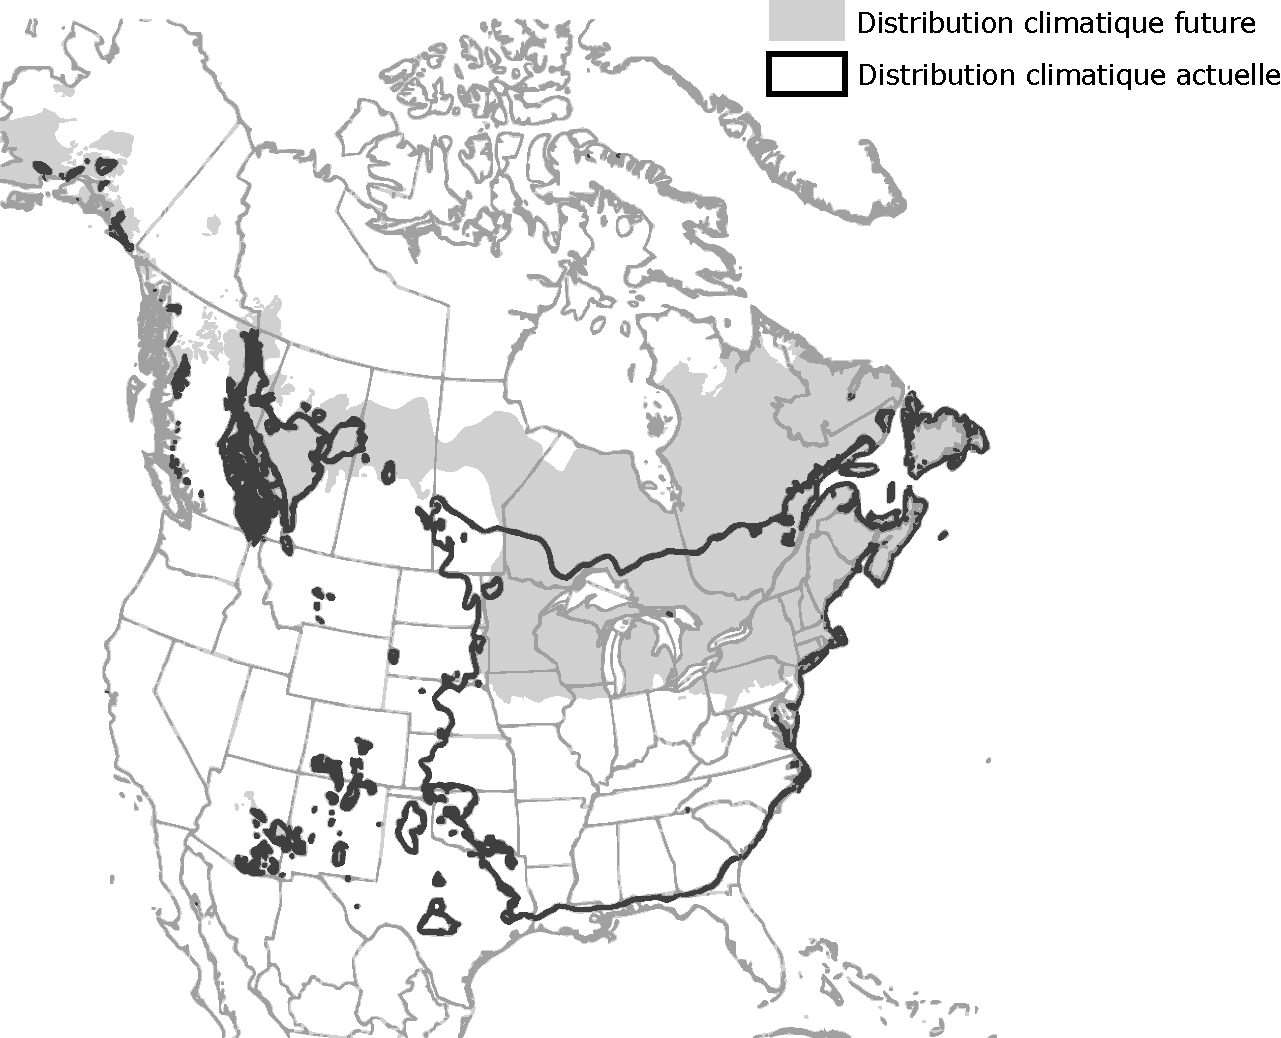
\includegraphics[scale=0.4]{figures/mckenney.pdf}\par

\smallcitation{McKenney et al. 2007 BioScience}

\end{frame}

\begin{frame}{La forêt ne suit pas les changements climatiques}

\centering
 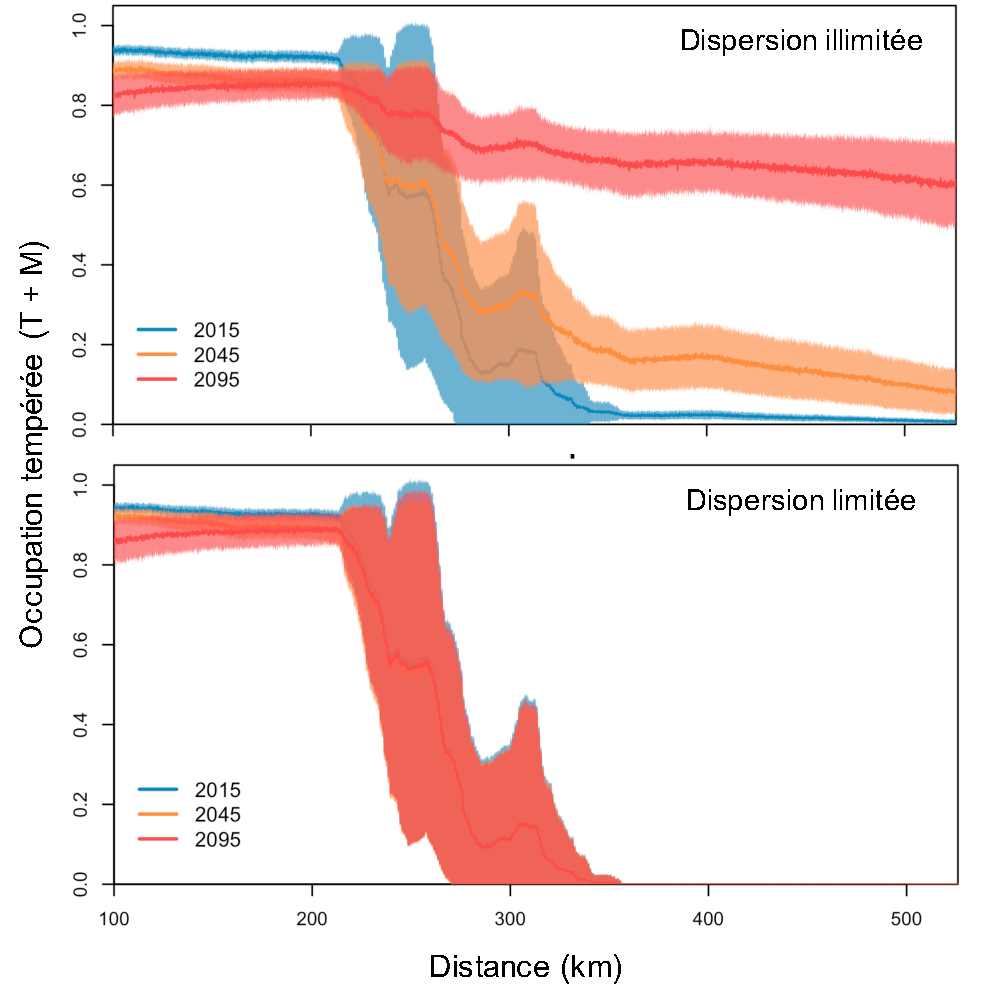
\includegraphics[scale=0.45]{figures/Vissault.pdf}\par

\smallcitation{Vissault et al. submitted}

\end{frame}

\begin{frame}{Possibles conséquences}

\begin{center}
  \begin{tikzpicture}
    \node<1> (img1) {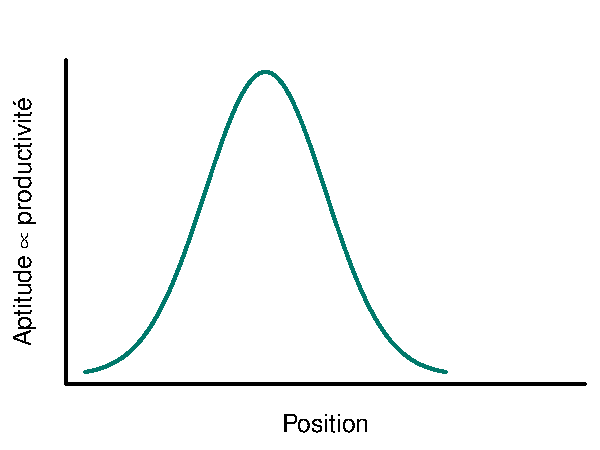
\includegraphics[scale=0.85]{figures/niche1.pdf}};
    \node<2> (img2) {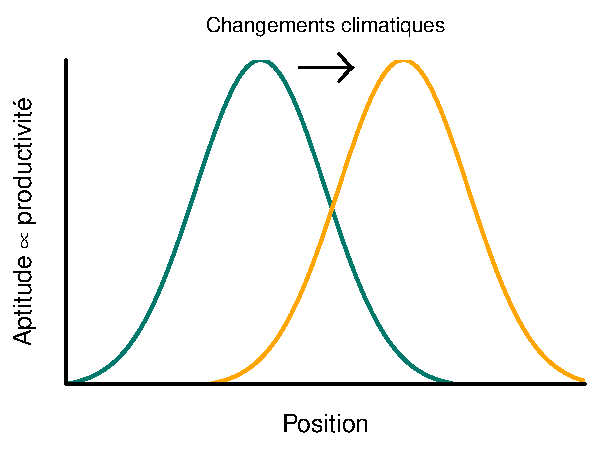
\includegraphics[scale=0.85]{figures/niche2.pdf}};
    \node<3> (img3) {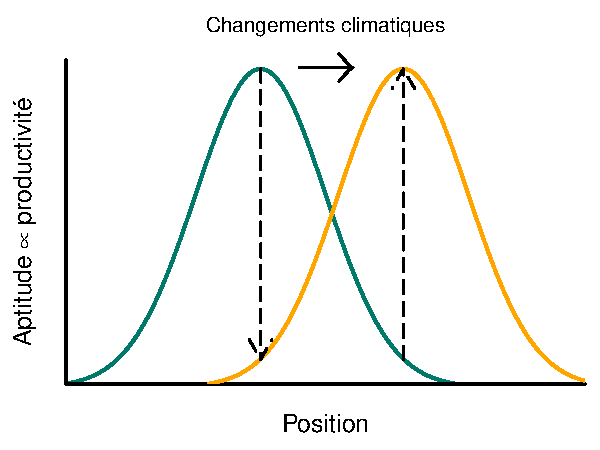
\includegraphics[scale=0.85]{figures/niche3.pdf}};
  \end{tikzpicture}
\end{center}

\end{frame}

\begin{frame}{Solution?}

\begincols
\column{0.28\textwidth}

\textbf{Aménagement forestier}

\begin{enumerate}
    \def\labelenumi{\arabic{enumi}.}
    \tightlist
    \item
      Plantation
    \item
      Coupe
    \item
      Eclaircie
    \item
      Enrichissement
  \end{enumerate}

\centering{Aménagement \newline X \newline processus écologiques}
\hfill\column{0.55\textwidth} \centering
 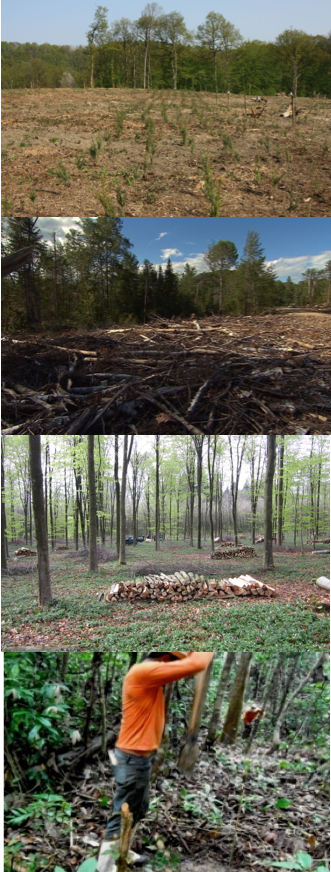
\includegraphics[scale=0.50]{figures/managPrac}\par
\stopcols

\end{frame}

\begin{frame}{Cadre théorique - expansion des espèces}

\begin{LARGE}
$$ 2 \times \sqrt{rD} $$
\end{LARGE}

\begin{description}
\tightlist
\item[r]
taux de croissance de la population
\item[D]
coefficient de diffusion
\end{description}

\smallcitation{Fisher 1937 Ann. Eugenics, Skellam 1951 Biometrika}

\end{frame}

\begin{frame}{Cadre théorique - interactions interspécifiques}

\centering
 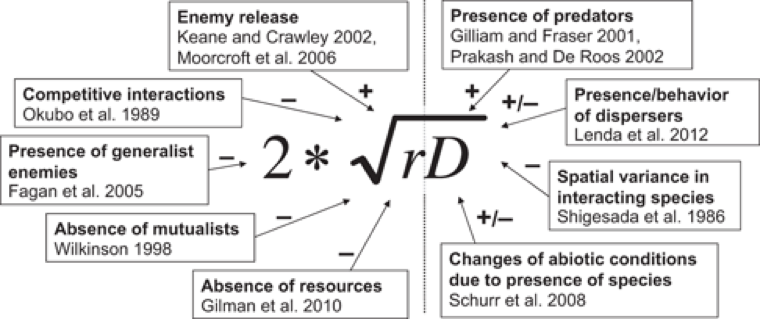
\includegraphics[scale=0.8]{figures/Svenning2014.png}\par

\smallcitation{Svenning et al. 2014 Ecography}

\end{frame}

\begin{frame}{Cadre théorique - Intégration de l'aménagement forestier}

\centering
 \begin{center}
  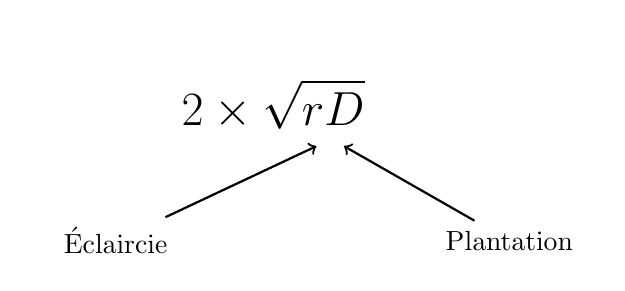
\begin{tikzpicture}[thick,every text node part/.style={align=center}]

    % --------------------------------------------------------- %
    % ------------- principal node (Formula)
    % --------------------------------------------------------- %
    \node[text width=6cm,minimum height=1cm,minimum width=3cm] (formule) at (10,10) {\LARGE{$$2 \times \sqrt{rD}$$}};

    % --------------------------------------------------------- %
    % ------------ Effect of forst management
    % --------------------------------------------------------- %
    \node[text width=2cm] (ecl) at (8,8) {Éclaircie};
    \draw[->]	(ecl) to node [midway] (formule) {} (10.55,9.2);

    \node[text width=2cm] (plant) at (13,8) {Plantation};
    \draw [->] (plant) to node [midway] (formule) {} (10.9,9.2);

  \end{tikzpicture}
\end{center}
\par

\end{frame}

\section{\texorpdfstring{Intégrer l'aménagement forestier \newline au
sein de modèles théoriques afin de mieux prédire la distribution
\newline et la productivité des espèces dans un contexte de changements
\newline climatiques}{Intégrer l'aménagement forestier au sein de modèles théoriques afin de mieux prédire la distribution et la productivité des espèces dans un contexte de changements climatiques}}\label{intuxe9grer-lamuxe9nagement-forestier-au-sein-de-moduxe8les-thuxe9oriques-afin-de-mieux-pruxe9dire-la-distribution-et-la-productivituxe9-des-espuxe8ces-dans-un-contexte-de-changements-climatiques}

\section{\texorpdfstring{L'aménagement forestier peut-il
\newline augmenter l'adaptabilité de la forêt aux changements
climatiques
?}{L'aménagement forestier peut-il augmenter l'adaptabilité de la forêt aux changements climatiques ?}}\label{lamuxe9nagement-forestier-peut-il-augmenter-ladaptabilituxe9-de-la-foruxeat-aux-changements-climatiques}

\section{\texorpdfstring{Quels mécanismes, à l'échelle locale et
régionale, déterminent la réponse de la forêt aux changements
\newline climatiques
?}{Quels mécanismes, à l'échelle locale et régionale, déterminent la réponse de la forêt aux changements climatiques ?}}\label{quels-muxe9canismes-uxe0-luxe9chelle-locale-et-ruxe9gionale-duxe9terminent-la-ruxe9ponse-de-la-foruxeat-aux-changements-climatiques}

\section{Y a-t-il des interactions entre ces échelles spatiales
?}\label{y-a-t-il-des-interactions-entre-ces-uxe9chelles-spatiales}

\begin{frame}{Organisation des chapitres}

\vspace*{-15mm}
\begin{center}
  \hspace*{-12mm}
  \begin{tikzpicture}[thick,every text node part/.style={align=center}]

    % --------------------------------------------------------- %
    % ------------- principal node (question)
    % --------------------------------------------------------- %
    \node[text width=15cm] (question) at (10,10.25) {\textbf{\large Intégrer l'aménagement forestier et les interactions entre espèces au sein des modèles théoriques afin de mieux prédire la distribution et la productivité des espèces}};

    % --------------------------------------------------------- %
    % ------------ Objectives
    % --------------------------------------------------------- %
    % --- Obj0 node
    \node[text width=12cm,visible on=<2->] (obj0) at (10,8.75) {L'aménagement forestier peut-il augmenter le taux de migration de la forêt vers le nord ?};
    \draw [->,visible on=<2->] (question) edge [out=270, in=90] (obj0);
    % --- Obj1 node
    \node[text width=12cm,visible on=<3->] (obj1) at (10,7.25) {Quelle est l'effet du climat, de l'interactions entre espèces et de l'aménagement forestier sur la démographie des arbres ?};
    \draw [->,visible on=<3->] (obj0) edge [out=270, in=90] (obj1);
    % --- Obj2 node
    \node[text width=9cm,visible on=<4->] (obj2) at (6.5,5.25) {Quand et comment les interactions biotiques sont plus importantes que le climat pour définir la limite de l'aire de répartition ?};
    \draw [->,visible on=<4->] (obj1) edge [out=195, in=90] (obj2);
    % --- Obj2 node
    \node[text width=8cm,visible on=<5->] (obj3) at (13.5,5.25) {Quand l'aménagement forestier peut-il impacter la performance des arbres à la limite d'aire de répartition ?};
    \draw [->,visible on=<5->] (obj1) edge [out=345, in=90] (obj3);
    % --- Obj3 node

  \end{tikzpicture}
\end{center}


\end{frame}

\section{\texorpdfstring{Chapitre I: \newline L'aménagement forestier
peut-il \newline augmenter l'adaptabilité de la forêt de l'est de
l'Amérique du Nord aux changements climatiques
?}{Chapitre I: L'aménagement forestier peut-il augmenter l'adaptabilité de la forêt de l'est de l'Amérique du Nord aux changements climatiques ?}}\label{chapitre-i-lamuxe9nagement-forestier-peut-il-augmenter-ladaptabilituxe9-de-la-foruxeat-de-lest-de-lamuxe9rique-du-nord-aux-changements-climatiques}

\begin{frame}{Contexte - objectif}

\begin{center}
  \begin{tikzpicture}
    \node<1> (img1) {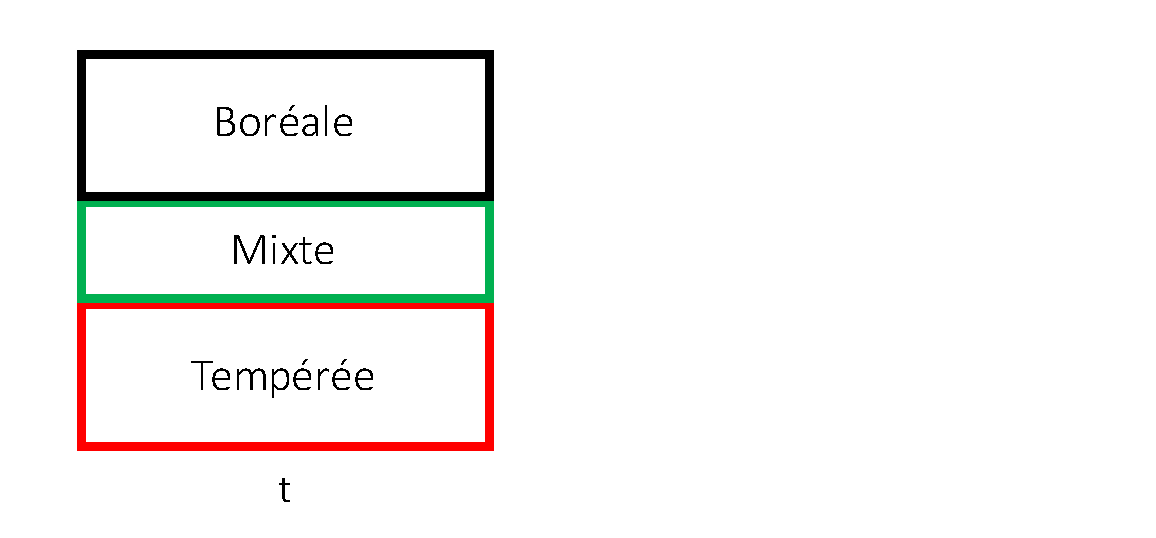
\includegraphics[scale=0.65]{figures/migration0.pdf}};
    \node<2> (img2) {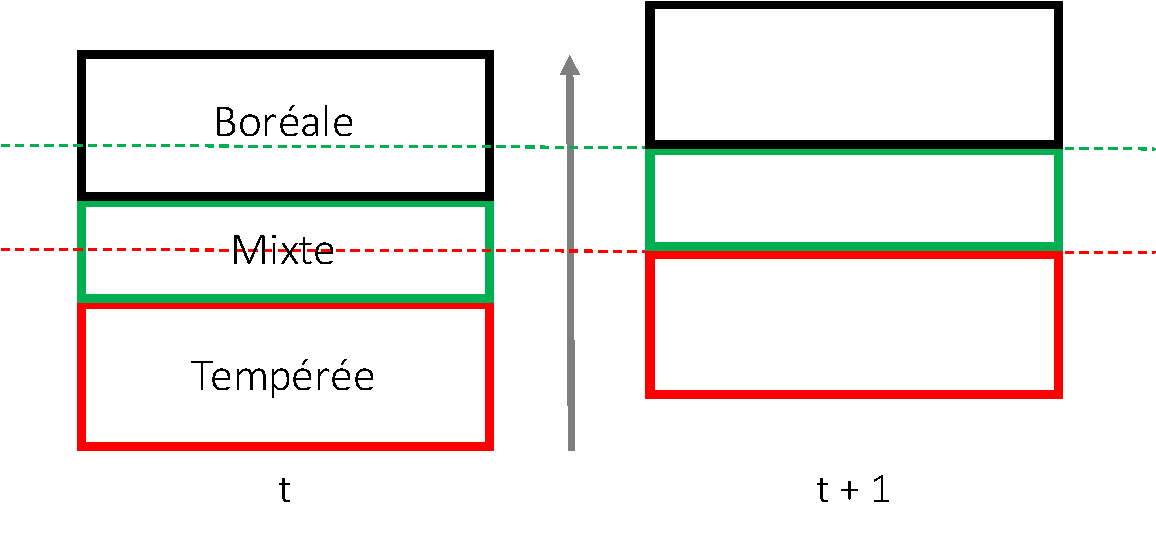
\includegraphics[scale=0.65]{figures/migration.pdf}};
    \node<3> (img3) {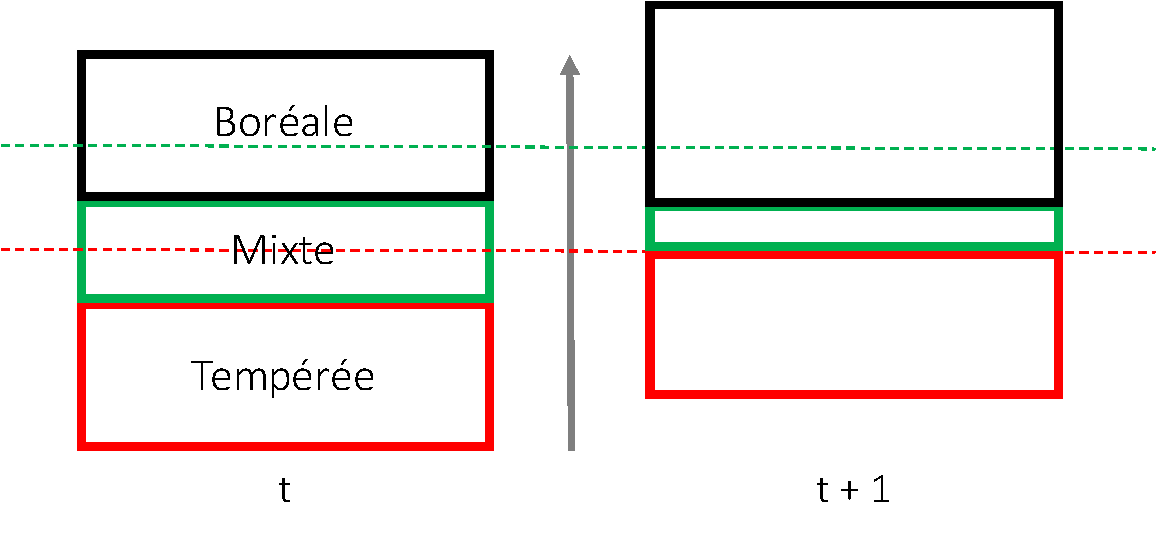
\includegraphics[scale=0.65]{figures/migration1.pdf}};
    \node<4> (img4) {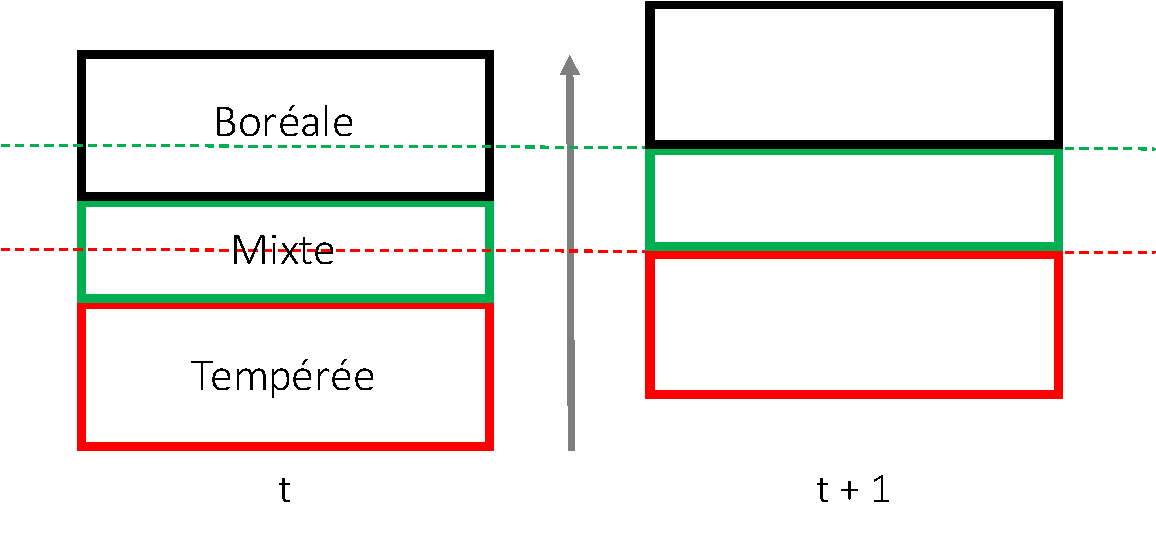
\includegraphics[scale=0.65]{figures/migration.pdf}};
  \end{tikzpicture}
\end{center}

\end{frame}

\begin{frame}{Modèle}

\begincols
\column{0.48\textwidth} 	\begin{tikzpicture}[->,>=stealth',auto,scale=0.45]
		\node [circle,StateM] (M) at (0,0) {\textcolor{white}{M}};
		\node [circle,StateB] (B) at (-8,5) {\textcolor{white}{B}};
		\node [circle,StateT] (T) at (8,5) {\textcolor{white}{T}};
		\node [circle,StateR] (R) at (0,10) {\textcolor{white}{R}};

		\path	(M) edge [thick,loop below,-latex]  node {} (M);
		\path	(T) edge [thick,loop right,-latex]  node {} (T);
		\path	(B) edge [thick,loop left,-latex]  node {} (B);
		\path	(R) edge [thick,loop above,-latex]  node {} (R);

		\draw[thick,-latex] (M) to node[above,sloped] {} (B);
		\draw[thick,-latex] (B) to[bend right=25] node[below,sloped] {} (M);

		\draw[thick,-latex] (T) to[bend left=25] node[below,sloped] {Colonisation} (M);
		\draw[thick,-latex] (M) to node[above,sloped] {Exclusion compétitive} (T);

		\draw[thick,-latex] (R) to[bend left=25] node[above,sloped] {Succession} (T);
		\draw[thick,-latex] (T) to node[below,sloped] {Pertubation} (R);

		\draw[thick,-latex] (R) to[bend right=25] node[above,sloped] {} (B);
		\draw[thick,-latex] (B) to node[below,sloped] {} (R);

		\draw[thick,-latex,transform canvas={xshift=0.8ex}] (R) to node[above,sloped] {} (M);
		\draw[thick,-latex,transform canvas={xshift=-0.8ex}] (M) to node[above,sloped] {} (R);
	\end{tikzpicture}

\hfill\column{0.35\textwidth}

\begin{description}
\tightlist
\item[B]
Boréale
\item[M]
Mixte
\item[T]
Tempérée
\item[R]
Régeneration
\end{description}

\stopcols

\end{frame}

\begin{frame}{Intégration avec l'aménagement forestier}

\centering
 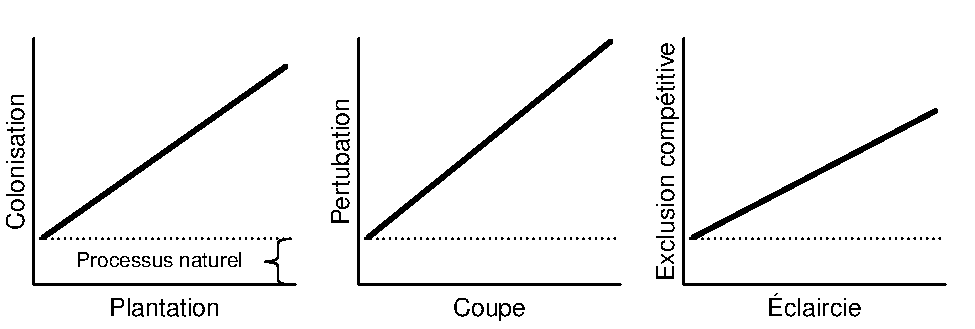
\includegraphics[scale=0.65]{figures/managMechanism.pdf}\par

\end{frame}

\begin{frame}{Résultats préliminaires}

Effet de la \textbf{plantation} et de la \textbf{coupe}

\centering
 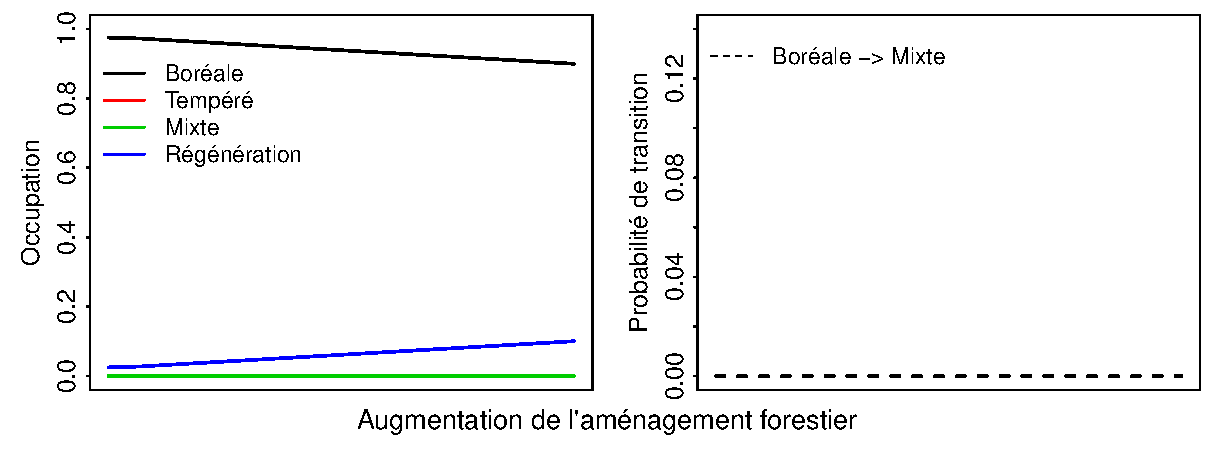
\includegraphics[scale=0.65]{figures/result0.pdf}\par

\end{frame}

\begin{frame}{Résultats préliminaires}

Effet de l'\textbf{éclaircie}

\centering
 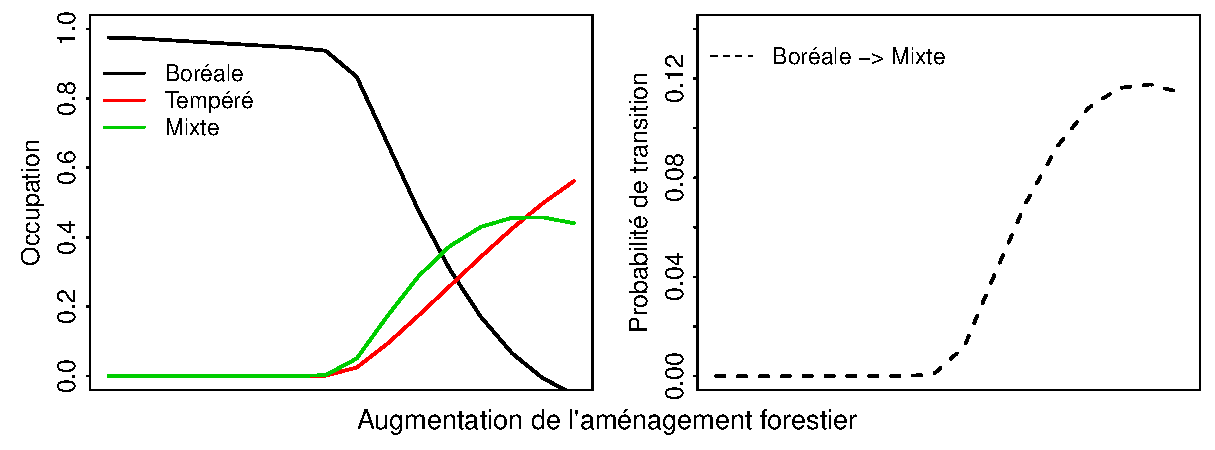
\includegraphics[scale=0.65]{figures/result1.pdf}\par

\end{frame}

\begin{frame}{Dynamiques forestières à différentes échelles spatiales}

\begin{columns}[T]
  \column{6.5cm}
    1. Locale

    \centering
      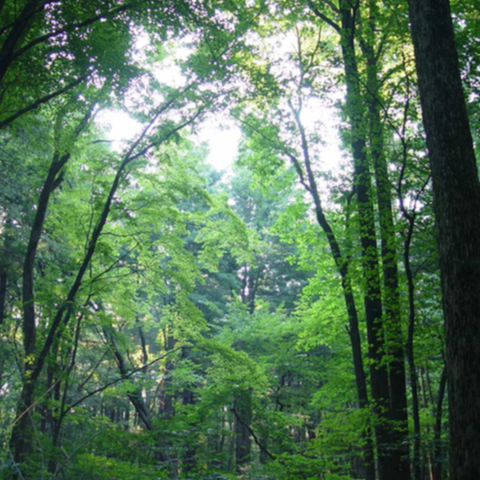
\includegraphics[scale=0.338]{figures/gap}\par
  \column{6.5cm}
    2. Régionale

    \centering
      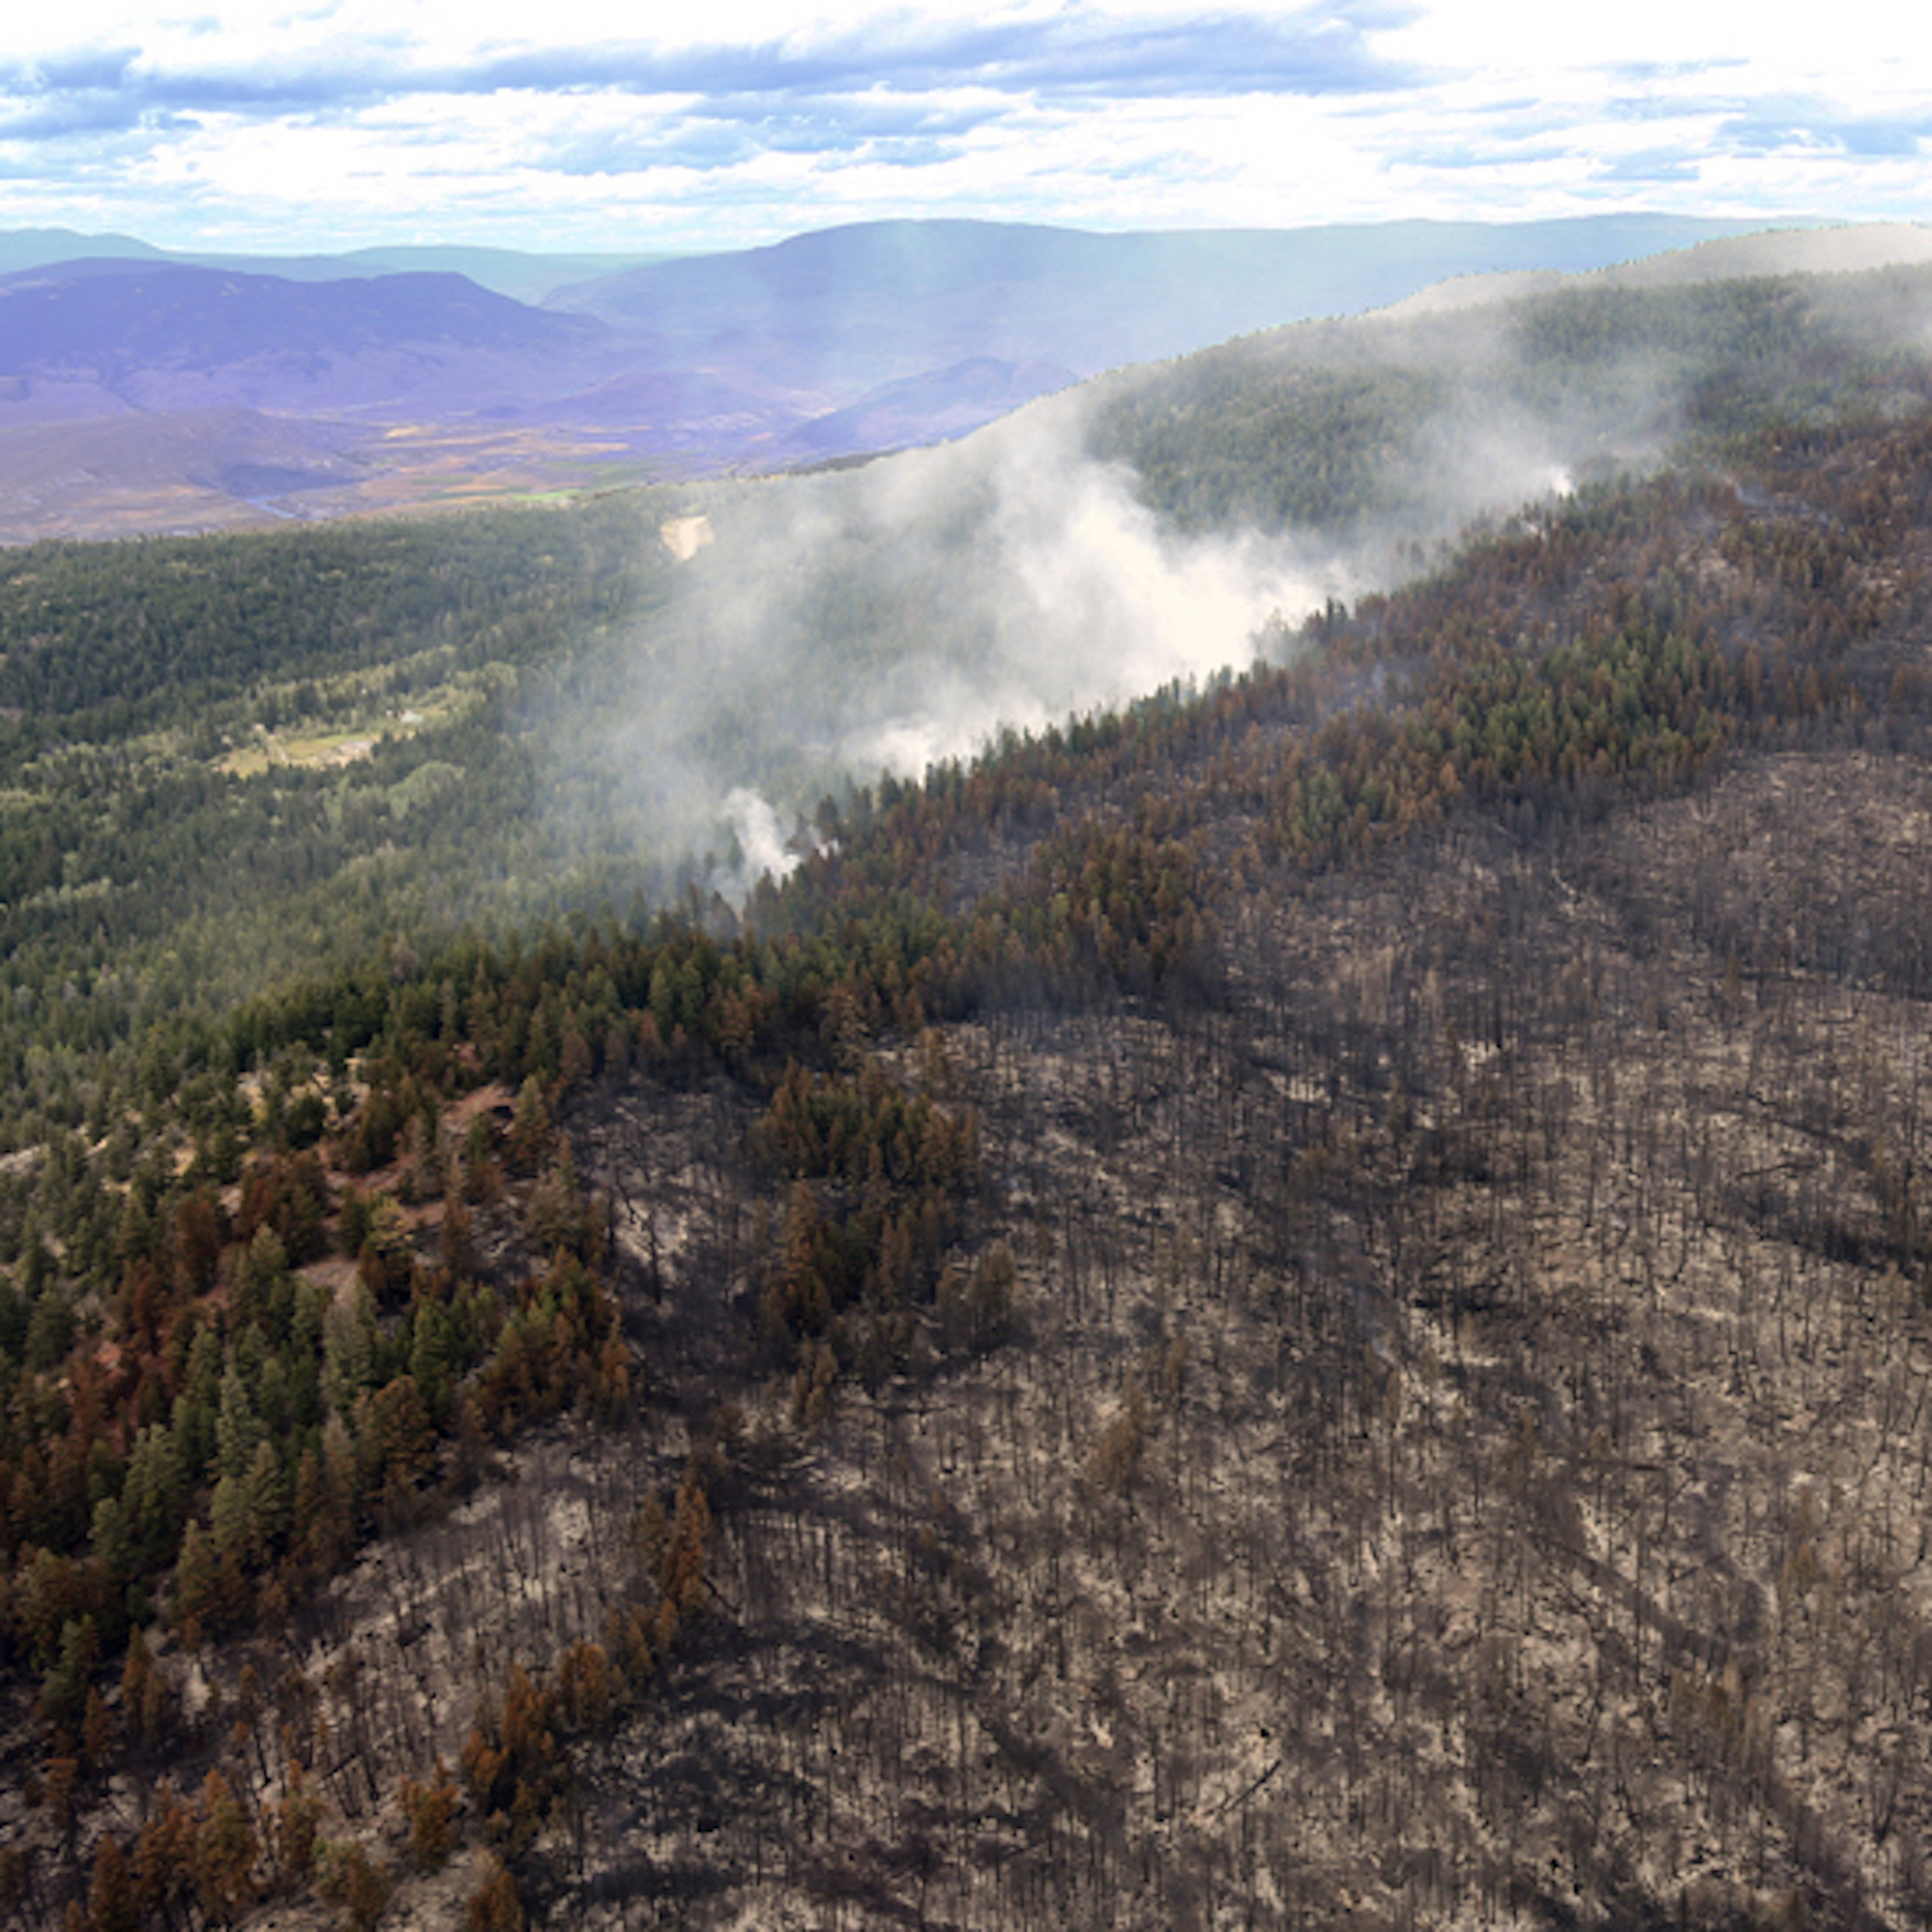
\includegraphics[scale=0.08]{figures/fire}\par
\end{columns}

\end{frame}

\begin{frame}{Aménagement forestier à différentes échelles spatiales}

Éclaircie

\centering
 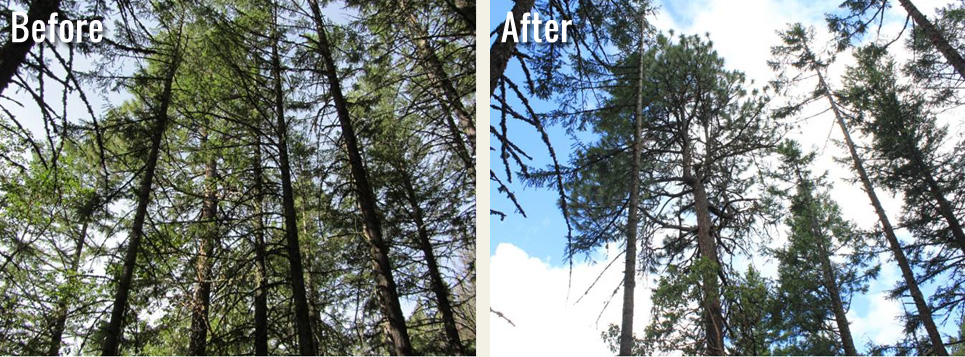
\includegraphics[scale=0.338]{figures/thinning}\par

\end{frame}

\begin{frame}{Aménagement forestier à différentes échelles spatiales}

Plan de gestion

\centering
 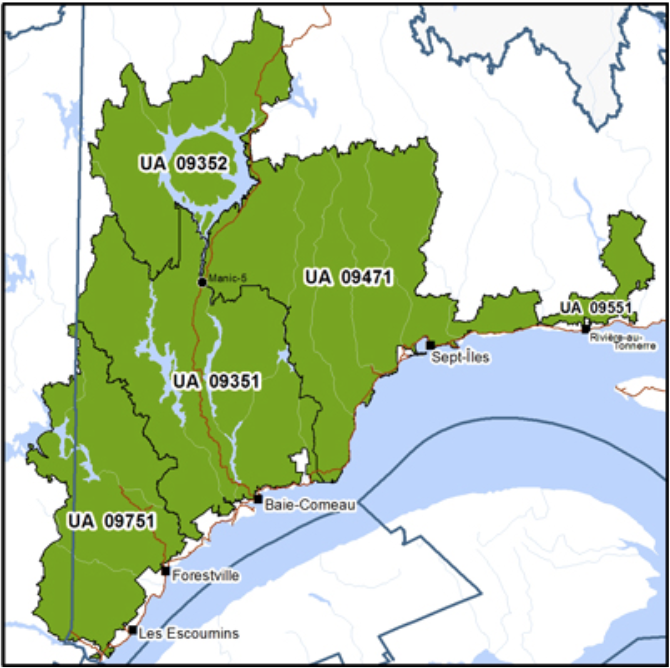
\includegraphics[scale=0.28]{figures/planGestion}\par

\end{frame}

\section{\texorpdfstring{Chapitre II et III: \newline Quels mécanismes,
à l'échelle locale et régionale, déterminent la réponse des forêts aux
changements climatiques
?}{Chapitre II et III: Quels mécanismes, à l'échelle locale et régionale, déterminent la réponse des forêts aux changements climatiques ?}}\label{chapitre-ii-et-iii-quels-muxe9canismes-uxe0-luxe9chelle-locale-et-ruxe9gionale-duxe9terminent-la-ruxe9ponse-des-foruxeats-aux-changements-climatiques}

\begin{frame}{Importance des interactions entre échelles spatiales}

\begincols
\column{0.40\textwidth}

\begin{enumerate}
    \def\labelenumi{\arabic{enumi}.}
    \tightlist
    \item
      Différents processus à différentes échelles
    \item
      Local -> Régionale
  \end{enumerate}

\hfill\column{0.55\textwidth} \centering
 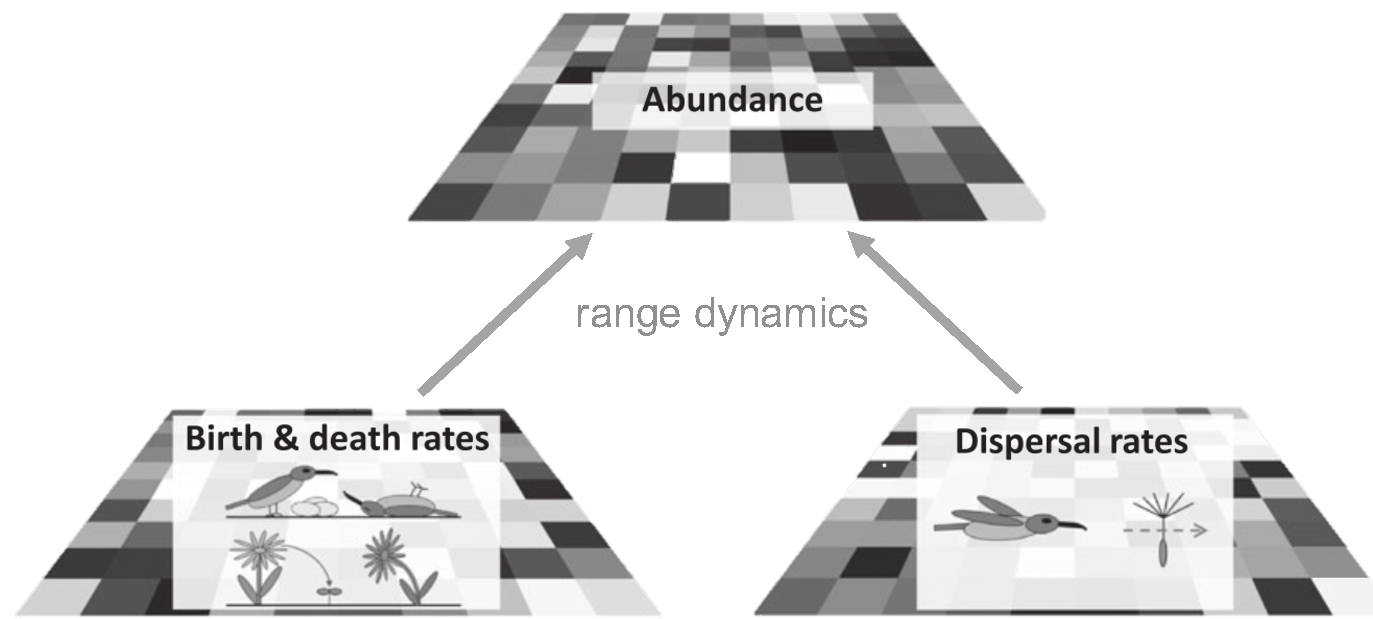
\includegraphics[scale=0.35]{figures/scaleInteg.pdf}\par
\stopcols
\smallcitation{Schurr et al. 2012 J. Biogeogr.}

\end{frame}

\section{Chapitre IV: Y a-t-il des interactions entre ces échelles
spatiales
?}\label{chapitre-iv-y-a-t-il-des-interactions-entre-ces-uxe9chelles-spatiales}

\begin{frame}{Modèle structuré à l'échelle locale}

\begincols
\column{0.18\textwidth}

\begin{enumerate}
    \def\labelenumi{\arabic{enumi}.}
    \tightlist
    \item
      Survie
    \item
      Croissance
    \item
      Reproduction
  \end{enumerate}

\hfill\column{0.55\textwidth} \centering
 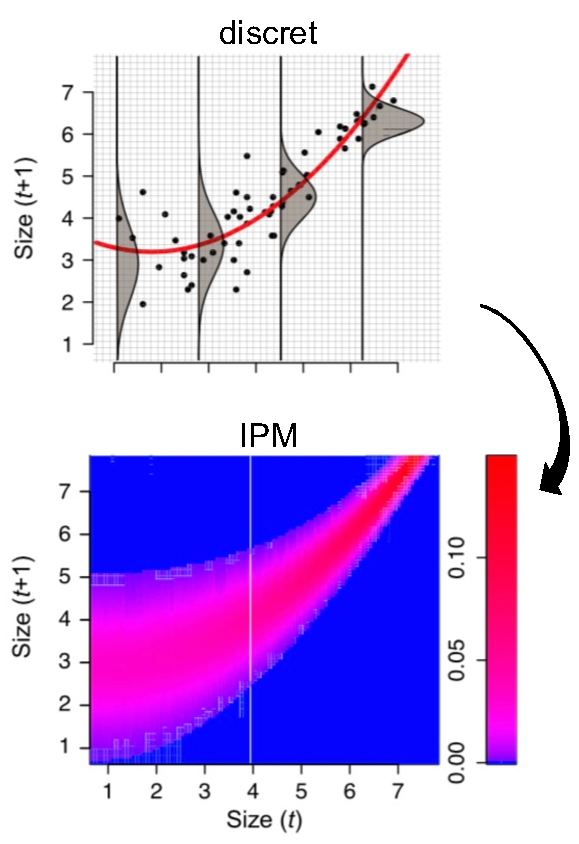
\includegraphics[scale=0.50]{figures/IPM}\par
\stopcols

\end{frame}

\begin{frame}{Approche hiérarchique}

\centering
 \begin{center}
    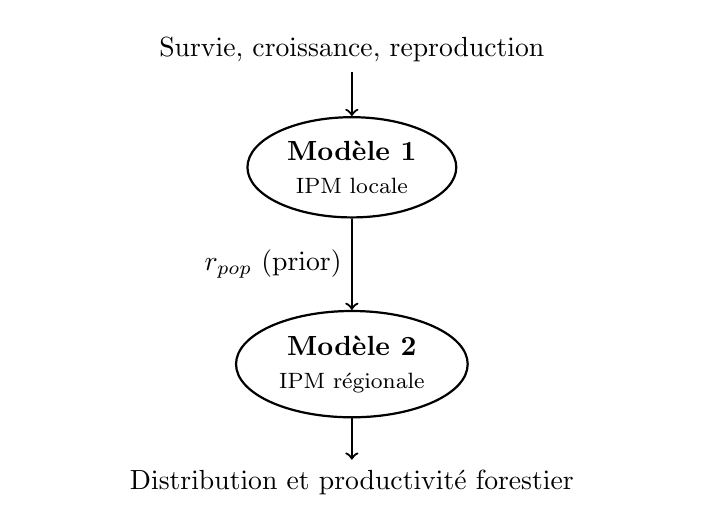
\begin{tikzpicture}[thick,every text node part/.style={align=center}]

    % --- model 1 node
    \node[draw, ellipse] (model1) at (10, 10) {\textbf{Modèle 1} \\ \footnotesize{IPM locale}};
    % --- model 2 node
    \node[draw, ellipse] (model2) at (10, 7.5) {\textbf{Modèle 2} \newline \\ \footnotesize{IPM régionale}};
    \draw[thick,->] (model1) -- (model2) node[midway,sloped,left,rotate=90] {$r_{pop}$ (prior)};

    % --- Structure
    \node[text width=6cm] (struc) at (10,11.5) {Survie, croissance, reproduction};
    \draw [->] (struc) edge (model1);
    % --- Distribution des espèces
    \node[text width=8cm] (dist) at (10,6) {Distribution et productivité forestier};
    \draw [->] (model2) edge (dist);

  \end{tikzpicture}
\end{center}
\par
\smallcitation{Talluto et al. 2016 Glob. Ecol. Biogeogr.}

\end{frame}

\section{Conclusion}\label{conclusion}

\begin{frame}{Contribution du projet}

\begin{enumerate}
\def\labelenumi{\arabic{enumi}.}
\tightlist
\item
  Meilleure compréhension des processus écologiques X aménagement
  forestier
\item
  Intégration des échelles spatiales
\item
  Prédiction plus précise des aires de répartition et productivité
  forestier
\end{enumerate}

\end{frame}

\begin{frame}[plain]{}

\plain{Merci !}

\end{frame}

\begin{frame}[plain]
  \begin{picture}(0,0)
    \put(-28.5,-175){%
      \pgfuseimage{titlebackground}
    }
  \end{picture}
\end{frame}

\end{document}
